\documentclass[11pt]{article}
\usepackage{amsmath,amsthm,amsfonts,amssymb,amscd}
\usepackage{multirow,booktabs}
\usepackage[table]{xcolor}
\usepackage{fullpage}
\usepackage{lastpage}
\usepackage{enumitem}
\usepackage{fancyhdr}
\usepackage{mathrsfs}
\usepackage{wrapfig}
\usepackage{setspace}
\usepackage{neuralnetwork}
\usepackage{calc}
\usepackage{multicol}
\usepackage{cancel}
\usepackage{tikz}
\usepackage{pgfplots}
\usepackage[retainorgcmds]{IEEEtrantools}
\usepackage[margin=3cm]{geometry}
\usepackage{amsmath}
\newlength{\tabcont}
\setlength{\parindent}{0.0in}
\setlength{\parskip}{0.05in}
\usepackage{empheq}
\usepackage{framed}
\usepackage[most]{tcolorbox}
\usepackage{xcolor}
\colorlet{shadecolor}{orange!15}
\parindent 0in
\parskip 12pt
\geometry{margin=1in, headsep=0.25in}
\theoremstyle{definition}
\newtheorem{defn}{Definition}
\newtheorem{reg}{Rule}
\newtheorem{exer}{Exercise}
\newtheorem{note}{Note}
\begin{document}
\title{Mathematical background for neural networks}

\thispagestyle{empty}

\begin{center}
{\LARGE \bf Mathematical background for neural networks}\\
\end{center}

\section{Mathematical background}
\subsection{Introduction}
Our neural network code is created with a modular design, where each layer of the 
network is an instance of its respective layer class, which inherits from the base 
class \texttt{Layer}. This allows for quick and easy creation and changes to the 
network architecture. To achieve this, however, we need to compute the loss gradient 
with repect to each layer regardless of the layer that came before it. We find that the 
chain rule tells us that all we need to compute the gradient of a given layer is the 
output gradient of that layer.
We can show this by the equation,
\begin{equation}
    \frac{\partial L}{\partial \mathbf{W}_i} = \frac{\partial L}{\partial \mathbf{Y}_i} \frac{\partial \mathbf{Y}_i}{\partial \mathbf{W}_i}
\end{equation}
where $L$ is the loss function, $\frac{\partial L}{\partial \mathbf{Y}_i}$ is the output 
gradient of layer $i$.
Since for layer $i$, the output $\mathbf{Y}_i$ is equal to the input $\mathbf{X}_{i+1}$ 
of the next layer $i+1$.
We also need to compute the input gradient with respect to each layer and return it for 
use of the previous layer, for which it becomes the output graident. 
\begin{equation}
    \frac{\partial L}{\partial \mathbf{Y}_i} = \frac{\partial L}{\partial \mathbf{X}_{i+1}} 
\end{equation}
\begin{figure}[h]
    \centering
    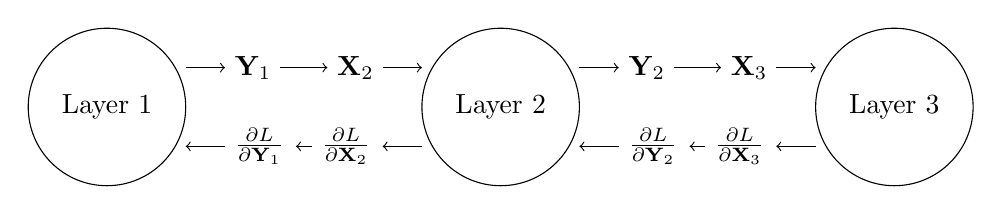
\begin{tikzpicture}
        % Define nodes
        \node[circle, draw, minimum size=2cm] (A) at (0,0) {Layer 1};
        \node[circle, draw, minimum size=2cm] (B) at (5,0) {Layer 2};
        \node[circle, draw, minimum size=2cm] (C) at (10,0) {Layer 3};

        % Connect nodes 1-2 forward
        \draw[->] (1,0.5) -- (1.5,0.5) node[right] {$\mathbf{Y}_1$};
        \draw[->] (2.2,0.5) -- (2.8,0.5) node[right] {$\mathbf{X}_2$};
        \draw[->] (3.5,0.5) -- (4,0.5);

        % Connect nodes 2-3 forward
        \draw[->] (6,0.5) -- (6.5,0.5) node[right] {$\mathbf{Y}_2$};
        \draw[->] (7.2,0.5) -- (7.8,0.5) node[right] {$\mathbf{X}_3$};
        \draw[->] (8.5,0.5) -- (9,0.5);

        % Connect nodes 3-2 backward
        \draw[<-] (6,-0.5) -- (6.5,-0.5) node[right] {$\frac{\partial L}{\partial \mathbf{Y}_2}$};
        \draw[<-] (7.4,-0.5) -- (7.6,-0.5) node[right] {$\frac{\partial L}{\partial \mathbf{X}_3}$};
        \draw[<-] (8.5,-0.5) -- (9,-0.5);

        % Connect nodes 2-1 backward
        \draw[<-] (1,-0.5) -- (1.5,-0.5) node[right] {$\frac{\partial L}{\partial \mathbf{Y}_1}$};
        \draw[<-] (2.4,-0.5) -- (2.6,-0.5) node[right] {$\frac{\partial L}{\partial \mathbf{X}_2}$};
        \draw[<-] (3.5,-0.5) -- (4,-0.5);
    \end{tikzpicture}
    \caption{Forward and backward pass of a neural network}
    \label{fig:forward_backward}
\end{figure}
\subsection{Fully Connected Layer}
\subsubsection{Forward Propagation}
Our dense or fully connected layer forward propagation is defined by the equation,
\begin{equation}
    \mathbf{Y} = \mathbf{W} \mathbf{X} + \mathbf{B}
\end{equation}
where $\mathbf{X}$ is the input, $\mathbf{W}$ is the weight matrix, $\mathbf{B}$ is the 
bias vector, and $\mathbf{Y}$ is the output. The weight matrix is of size $n \times m$ 
where $n$ is the number of output features and $m$ is the number of input features. 
The bias vector is of size $m$. If the input matrix is of size $m \times o$ where $o$ 
is the number of samples, then the output matrix is of size $n \times o$. 
We can write the $i$-th element of the $b$-th output vector in a batch of outputs as,
\begin{equation}
    y_i^{[b]} = \sum_{j=1}^{n} w_{i,j} x_j^{[b]} + b_i
    \label{eq:paticular_output}
\end{equation}
\subsubsection{Loss Gradient with respect to the Weight Matrix}
The error gradient with 
respect to the weigth matrix is given by,
\begin{equation}
    \frac{\partial L}{\partial \mathbf{W}} = \frac{\partial L}{\partial \mathbf{Y}} \frac{\partial \mathbf{Y}}{\partial \mathbf{W}}
\end{equation}
. Within our backward propagation method we are given the output gradient 
$\frac{\partial L}{\partial \mathbf{Y}}$ as an argument. This leaves us to compute 
$\frac{\partial \mathbf{Y}}{\partial \mathbf{W}}$. For any particular element of the 
gradient $\frac{\partial \mathbf{Y}}{\partial \mathbf{W}}$ we can substitute equation 
\ref{eq:paticular_output} into the equation,
\begin{equation}
    \frac{\partial y^{[b]}_t}{\partial w_{i,j}} = \frac{\partial}{\partial w_{i,j}} \left( \sum_{j=1}^{n} w_{t,j} x_j^{[b]} + b_t \right) = 
    \begin{cases}
        x_j^{[b]} & \text{if } i = t \\
        0 & \text{otherwise}
    \end{cases}
    \label{eq:dense_grad_particular}
\end{equation}
. Representing the gradient of the loss function with respect to the weight matrix as a
matrix, we have,
\begin{equation}
    \frac{\partial L}{\partial \mathbf{W}} = 
    \begin{bmatrix}
        \frac{\partial L}{\partial w_{1,1}} & \frac{\partial L}{\partial w_{1,2}} & \cdots & \frac{\partial L}{\partial w_{1,n}} \\
        \frac{\partial L}{\partial w_{2,1}} & \frac{\partial L}{\partial w_{2,2}} & \cdots & \frac{\partial L}{\partial w_{2,n}} \\
        \vdots & \vdots & \ddots & \vdots \\
        \frac{\partial L}{\partial w_{m,1}} & \frac{\partial L}{\partial w_{m,2}} & \cdots & \frac{\partial L}{\partial w_{m,n}}
    \end{bmatrix}
    \label{eq:dense_grad_matrix}
\end{equation}
. It follows from equation \ref{eq:dense_grad_particular} that the gradient of the loss 
function with respect a particular weight $w_{i,j}$ is given by,
\begin{equation}
    \frac{\partial L}{\partial w_{i,j}} = \sum_{b=1}^{o} \frac{\partial L}{\partial y^{[b]}_i} x_j^{[b]}
    \label{eq:dense_grad}
\end{equation}
. Substituting equation \ref{eq:dense_grad} into equation \ref{eq:dense_grad_matrix} we
find the that final gradient of the loss function with respect to the weight matrix is 
given by,
\begin{equation}
    \frac{\partial L}{\partial \mathbf{W}} = \frac{\partial L}{\partial \mathbf{Y}} \mathbf{X}^T
\end{equation}
\subsubsection{Loss Gradient with respect to the Bias Vector}
The error gradient with respect to the bias vector is given by,
\begin{equation}
    \frac{\partial L}{\partial \mathbf{B}} = \frac{\partial L}{\partial \mathbf{Y}} \frac{\partial \mathbf{Y}}{\partial \mathbf{B}}
\end{equation}
. Again, we are given the output gradient $\frac{\partial L}{\partial \mathbf{Y}}$ as 
an argument, so our task is to compute $\frac{\partial \mathbf{Y}}{\partial \mathbf{B}}$.
Referencing equation \ref{eq:paticular_output}, we can see that the gradient of the 
output with respect to the bias vector is given by,
\begin{equation}
    \frac{\partial y^{[b]}_i}{\partial b_j} = \frac{\partial}{\partial b_j} \left( \sum_{j=1}^{n} w_{i,j} x_j^{[b]} + b_i \right) = 
    \begin{cases}
        1 & \text{if } i = j \\
        0 & \text{otherwise}
    \end{cases}
\end{equation}
. Representing the gradient of the loss function with respect to the bias vector as a 
vector, we have,
\begin{equation}
    \frac{\partial L}{\partial \mathbf{B}} = 
    \begin{bmatrix}
        \frac{\partial L}{\partial b_1} \\[0.5em]
        \frac{\partial L}{\partial b_2} \\[0.5em]
        \vdots \\[0.5em]
        \frac{\partial L}{\partial b_m}
    \end{bmatrix}
\end{equation}
. It follows that the gradient of the loss function with respect to a particular bias 
$b_i$ is given by,
\begin{equation}
    \frac{\partial L}{\partial b_i} = \sum_{b=1}^{o} \frac{\partial L}{\partial y^{[b]}_i}
\end{equation}
which is simply the sum of the loss gradients with respect to the output.
\subsubsection{Loss Gradient with respect to the Input}
\subsection{Activation Functions}
Activation functions are used to introduce non-linearity into our neural network. We 
used a total of four activation functions in our code, the ReLU, Sigmoid, Tanh, and 
Softmax functions. Since all activation functions are not trainable, we only need to 
compute the input gradient. The input gradient is given by,
\begin{equation}
    \frac{\partial L}{\partial \mathbf{X}} = \frac{\partial L}{\partial \mathbf{Y}} \frac{\partial \mathbf{Y}}{\partial \mathbf{X}} 
    \label{eq:input_gradient_activation}
\end{equation}
. Hence, for each activation function we simply need to compute the derivative of the 
function with respect to the input.
\subsubsection{ReLU}
The ReLU function is defined as,
\begin{equation}
    f(x) = 
    \begin{cases}
        x & \text{if } x > 0 \\
        0 & \text{otherwise}
    \end{cases}
\end{equation}
\begin{figure}[h]
    \centering
    \begin{tikzpicture}
        % Draw axes
        \draw[->] (-2,0) -- (2,0) node[right] {$x$};
        \draw[->] (0,-1) -- (0,2) node[above] {$ReLU(x)$};
        
        % Plot ReLU function
        \draw[thick,blue] (-2,0) -- (0,0);
        \draw[thick,blue] (0,0) -- (2,2);
        
        % Add labels
        \node[left] at (-2,0) {$0$};
    \end{tikzpicture}    \caption{ReLU function}
    \label{fig:relu}
\end{figure}\\
Following equation \ref{eq:input_gradient_activation}, the input gradient is given by,
\begin{equation}
    \frac{\partial L}{\partial \mathbf{X}} = 
    \frac{\partial L}{\partial \mathbf{Y}} f'(\mathbf{X}) = 
    \frac{\partial L}{\partial \mathbf{Y}}
    \begin{cases}
        1 & \text{if } x > 0 \\
        0 & \text{otherwise}
    \end{cases}
\end{equation}
\subsubsection{Sigmoid}
The sigmoid function is defined as,
\begin{equation}
    f(x) = \frac{1}{1 + e^{-x}}
\end{equation}
\begin{figure}[h]
    \centering
    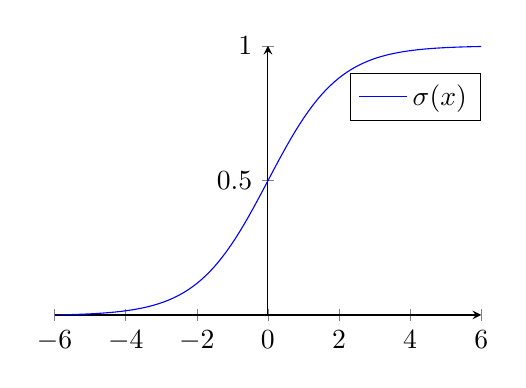
\begin{tikzpicture}[declare function={sigma(\x)=1/(1+exp(-\x));}]
    \begin{axis}%
    [
        height=5cm,
        width=7cm,
        xmin=-6,
        xmax=6,
        axis x line=bottom,
        ytick={0,.5,1},
        ymax=1,
        axis y line=middle,
        samples=100,
        domain=-6:6,
        legend style={at={(1,0.9)}}     
    ]
        \addplot[blue,mark=none]   (x,{sigma(x)});
        \legend{$\sigma(x)$}
    \end{axis}
    \end{tikzpicture}
    \caption{Sigmoid function}
    \label{fig:sigmoid}
\end{figure}\\
The derivative of the sigmoid function is given by,
\begin{equation}
    f'(x) = f(x)(1 - f(x))
\end{equation}
Hence, the input gradient is given by,
\begin{equation}
    \frac{\partial L}{\partial \mathbf{X}} = 
    \frac{\partial L}{\partial \mathbf{Y}} f'(\mathbf{X}) = 
    \frac{\partial L}{\partial \mathbf{Y}} f(\mathbf{X})(1 - f(\mathbf{X}))
\end{equation}
\subsubsection{Tanh}
The tanh function is defined as,
\begin{equation}
    f(x) = \frac{e^x - e^{-x}}{e^x + e^{-x}}
\end{equation}
\begin{figure}[h]
    \centering
    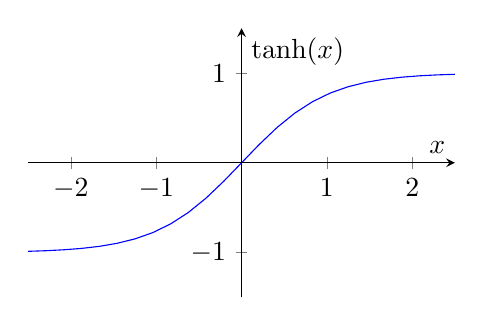
\begin{tikzpicture}[declare function={sigma(\x)=(exp(\x)-exp(-\x))/(exp(\x)+exp(-\x));}]
    \begin{axis}[
        width=7cm,
        height=5cm,
        xmin=-2.5, xmax=2.5,
        ymin=-1.5, ymax=1.5,
        axis lines=center,
        axis on top=true,
        domain=-2.5:2.5,
        ylabel=$\tanh(x)$,
        xlabel=$x$,
        ]
        \addplot[blue,mark=none]   (x,{sigma(x)});
    \end{axis}
    \end{tikzpicture}
    \caption{Tanh function}
    \label{fig:tanh}
\end{figure}\\
The derivative of the tanh function is given by,
\begin{equation}
    f'(x) = 1 - f(x)^2
\end{equation} 
Hence, the input gradient is given by,
\begin{equation}
    \frac{\partial L}{\partial \mathbf{X}} = 
    \frac{\partial L}{\partial \mathbf{Y}} f'(\mathbf{X}) = 
    \frac{\partial L}{\partial \mathbf{Y}} (1 - f(\mathbf{X})^2)
\end{equation}
\subsubsection{Softmax}
The softmax function is a unique activation function, that usually is only used on the 
output layer of a neural network. The softmax function is used to convert the output of 
a layer into a probability distribution. This is incredibly useful for classification 
problems. The softmax function is used on a vector of $n$ elements, and is defined as,
\begin{equation}
    f(x_i) = \frac{e^{x_i}}{\sum_{j=1}^{n} e^{x_j}}
\end{equation}
where $x_i$ is the $i$-th component of the vector and $f(x_i)$ is the probability of the $i$-th component of the vector.
\subsection{Convolutional Layer}
\subsubsection{Forward Propagation}
The convolutional layer is a layer that takes a 3 dimensional input, where the first 
two dimensions are the height and width of the input (usually pixel values of an 
image), and the third dimension is the of channels of the input. The convolutional 
layer is defined by the equation,
\begin{equation}
    \mathbf{Y}_{i}^{[b]} = \sum_{j=1}^n \mathbf{X}_{j}^{[b]} \ast  \mathbf{F}_{j,i} + \mathbf{B}_{i}
\end{equation}
where $\mathbf{Y}_{i}^{[b]}$ is the $i$-th channel of the $b$-th sample of the output , 
$\mathbf{X}_{j}^{[b]}$ is the $j$-th channel of the $b$-th sample of the input, 
$\mathbf{F}_{j,i}$ is the $j$-th channel of the $i$-th filter, $\mathbf{B}_{i}$ is the 
$i$-th bias vector and $\ast$ is the convolution operator. The convolution operator 
takes two 2-dimensional matrices and performs the following operation,
\section{Loss Functions}
\subsection{Mean Squared Error}
The mean squared error is defined as,
\begin{equation}
    L = \frac{1}{o} \sum_{i=1}^{o} \sum_{j=1}^{n} (y_{i,j} - \hat{y}_{i,j})^2
\end{equation}
where $o$ is the number of samples, $n$ is the number of output features, $y_{i,j}$ is 
the $j$-th component of the $i$-th sample, and $\hat{y}_{i,j}$ is the $j$-th predicted 
component of the $i$-th sample. The derivative of the loss function with respect to the 
final output ($\mathbf{\hat{Y}}$) is given by,
\begin{equation}
    \frac{\partial L}{\partial \mathbf{\hat{Y}}} = \frac{2}{o} (\mathbf{\hat{Y}} - \mathbf{Y})
\end{equation}
. The output of this function is then passed to the output layer for back propagation.
The mean squared error loss function is used extensively for regression problems.
\subsection{Cross Entropy}
The cross entropy loss function is defined as,
\begin{equation}
    L = -\frac{1}{o} \sum_{b=1}^{o} \sum_{i=1}^{n} y_{i}^{[b]} \log(\hat{y}_{i}^{[b]})
\end{equation}
where $o$ is the number of samples, $n$ is the number of output features, $y_{i}^{[b]}$
is the $i$-th component of the $b$-th sample, and $\hat{y}_{i}^{[b]}$ is the $i$-th 
predicted component of the $b$-th sample. The cross entropy loss function is used
primarily for classification problems. Since the softmax activation function is often
found on the output layer of a classification network, it is useful to compute the 
derivative of the loss function with respect to a softmaxed output. Considering 
a softmaxed output, the loss function becomes,
\begin{equation}
    L = -\frac{1}{o}\sum_{b=1}^{o}\sum_{i=1}^{n}y_{i}^{[b]}\log(\text{Softmax}(z^{[b]}_{i}))
\end{equation}
where $z^{[b]}_{i}$ is the $i$-th component of the $b$-th sample of the output of the
non-softmaxed output layer.
Looking at just the the loss function for a single sample, we can see that the 
derivative with respect to the output layer is:
\begin{align*}
    L_{i} &= -\sum_{j=1}^{10}y_{j}\log(a_{j}) \\
    \frac{\partial L_{i}}{\partial z^{[2]}_{i}} &= - \sum_{k=1}^{10}y_{k}\frac{\partial
        \log(a_{k})}{\partial z^{[2]}_{i}} \\
    &= - \sum_{k=1}^{10}y_{k}\frac{1}{a_{k}}\frac{\partial a_{k}}{\partial z^{[2]}_{i}} \\
\end{align*}
The derivative of the softmax function is:
\begin{equation}
    \frac{\partial a_{k}}{\partial z^{[2]}_{i}} = \begin{cases}
        a_{k}(1-a_{k}) & \text{if } k = i \\
        -a_{k}a_{i} & \text{if } k \neq i
    \end{cases}
\end{equation}
Hence:
\begin{align*}
    \frac{\partial L_{i}}{\partial z^{[2]}_{i}} &= -y_{j}(1-a_{j}) - \sum_{k \neq j}y_{k}a_{j}\\
                                                &= a_{j} \left( y_{j} + \sum_{k \neq j}y_{k} \right) - y_{j} \\
\end{align*}
Since $\sum_{k}y_{k} = 1$ and $y_{j} + \sum_{k \neq i}y_{k} = 1$, we have:
\begin{equation}
    \frac{\partial L_
    {i}}{\partial z^{[2]}_{i}} = a_{j} - y_{j}
\end{equation}

Hence:
\begin{equation}
    \frac{\partial L}{\partial 
    Z} = \hat{Y} - Y
\end{equation}
\end{document}
